% !TEX TS-program = pdflatex
% !TEX encoding = UTF-8 Unicode

% This is a simple template for a LaTeX document using the "article" class.
% See "book", "report", "letter" for other types of document.

\documentclass[11pt]{article} % use larger type; default would be 10pt

\usepackage[utf8]{inputenc} % set input encoding (not needed with XeLaTeX)

%%% Examples of Article customizations
% These packages are optional, depending whether you want the features they provide.
% See the LaTeX Companion or other references for full information.

%%% PAGE DIMENSIONS
\usepackage{geometry} % to change the page dimensions
\geometry{a4paper} % or letterpaper (US) or a5paper or....
% \geometry{margin=2in} % for example, change the margins to 2 inches all round
% \geometry{landscape} % set up the page for landscape
%   read geometry.pdf for detailed page layout information

\usepackage{graphicx} % support the \includegraphics command and options

% \usepackage[parfill]{parskip} % Activate to begin paragraphs with an empty line rather than an indent

%%% PACKAGES
\usepackage{booktabs} % for much better looking tables
\usepackage{array} % for better arrays (eg matrices) in maths
\usepackage{paralist} % very flexible & customisable lists (eg. enumerate/itemize, etc.)
\usepackage{verbatim} % adds environment for commenting out blocks of text & for better verbatim
\usepackage{subfig} % make it possible to include more than one captioned figure/table in a single float
\usepackage[linesnumbered,ruled,vlined]{algorithm2e} 
\usepackage[noend]{algpseudocode}
\usepackage{amsmath}
\usepackage{chngcntr}
\usepackage{kbordermatrix}
% These packages are all incorporated in the memoir class to one degree or another...

%%% HEADERS & FOOTERS
\usepackage{fancyhdr} % This should be set AFTER setting up the page geometry
\pagestyle{fancy} % options: empty , plain , fancy
\renewcommand{\headrulewidth}{0pt} % customise the layout...
\lhead{}\chead{}\rhead{}
\lfoot{}\cfoot{\thepage}\rfoot{}

%%% SECTION TITLE APPEARANCE
\usepackage{sectsty}
\allsectionsfont{\sffamily\mdseries\upshape} % (See the fntguide.pdf for font help)
% (This matches ConTeXt defaults)

%%% ToC (table of contents) APPEARANCE
\usepackage[nottoc,notlof,notlot]{tocbibind} % Put the bibliography in the ToC
\usepackage[titles,subfigure]{tocloft} % Alter the style of the Table of Contents
\renewcommand{\cftsecfont}{\rmfamily\mdseries\upshape}
\renewcommand{\cftsecpagefont}{\rmfamily\mdseries\upshape} % No bold!

\counterwithin*{equation}{section}
\counterwithin*{equation}{subsection}

%%% END Article customizations

%%% The "real" document content comes below...

\title{Assignment 4}
\author{Brandon Smith \& Nicholas Grieco}
\date{December 13, 2017}

\begin{document}
\maketitle

\section*{Problem 1}
\subsection*{a + b)}
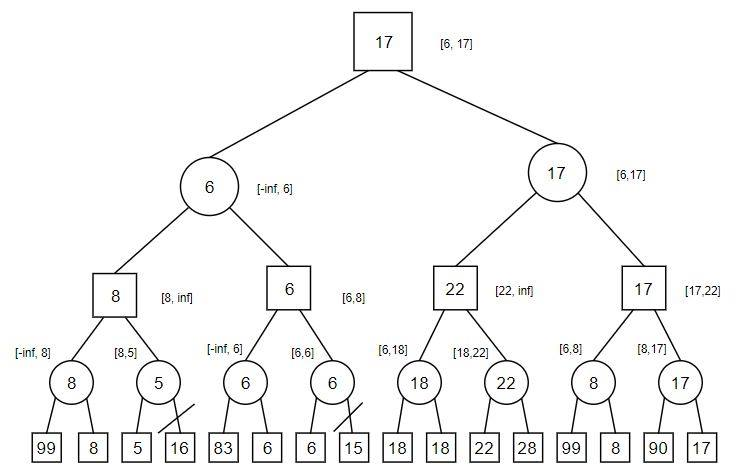
\includegraphics[scale=0.45]{prob1}
\subsection*{c)}
Exhaustive minimax and minimax with AB pruning will both choose the right move at the root node because it has the higher score given that both players play optimally every turn. Alpha-beta pruning does not affect the results of the adversarial search. AB pruning simply stops the search on nodes where it is known to not contain a solution. If the nodes are in a good order, the time complexity could be cut in half. Nodes are not always ordered in the best way which is why heuristic are used to reorder the nodes such that you can prune away as much as possible while still keeping a consistent solution.

\section*{Problem 2}

\subsection*{a.}
The variables are $n_{i,j}$ with each variable being part of a domain where  $ 0 < i < 8 $. The constraints are that each set of $n_{i,[0:8]}$ and $n_{[0:8],j}$ must be the set [1:9]. Furthermore the grid is divided into 9 subsections of 3x3 boxes. Each of these squares must contain the set [1:9]

\subsection*{b.}


Start State: The state where M grid cells are filled with numbers that satisfy the contraint. The start state grid would be the 9x9 grid with 81-M blank cells and M cells filled.\\

Successor Function: The successor function is placing one number on the grid in place of a blank cell.\\

Goal Test: The goal test would be to check every cell in the grid, so that no violations are found, and every cell contains a number\\
Cost Function: The cost function can be defined as the number of possible valid configurations in each blank cell minus the number of possible valid configurations after a cell is filled with a particular number.\\

The minimum remaining values heuristic would be better for solving this problem. The MRV heuristic is designed to be a ``fail-first'' heuristic and we are more likely to see a mistake earlier in the process because MRV chooses the node with the fewest possible values, compared to the degree heuristic which chooses the node with the most contraints.\\

The branching factor at each node is 9, because at each cell we have a total of 9 possible values that can be assigned. The depth to each solution would be the amount of tiles needed to solve the puzzle, so 81-M. The maximum depth of a search space would be 81 because the grid is 81 cells. Since the branching factor is 9, and the maximum depth of the tree is 81 the size of the state space will be $9^{81}$
\subsection*{c.}
An easy and hard puzzle would be the difference in the amounf of backtracking you need to do in order to solve the problem. A big factor in the amount of backtracking you do is depenent on the heuristic. Because the heuristic determines the cost it can change the order in which tiles are placed, changing the amount of backtracking that occurs. Consider the scenario where we have an optimal heuristic. The difference between a hard and easy puzzle will be determined by the amount of pre assigned numbers M. When M is higher we have more clues to solve the puzzle compared to when M is low and there is a lot of guessing that needs to be done. Therefor an easy puzzle is influenced by a higher M, and a hard puzzle is influenced by lower M.


\subsection*{d.}

\begin{algorithm}[H]
 \KwData{max-tries, grid with $M$ filled cells}
 \KwResult{A state where the puzzle is solved }
 \For{i := 0 to max-tries}{
  \uIf{grid is satisfied}{
    return grid\;
  }
	Choose random cell and change it to random state which maximizes heuristic\;
	  \uIf{heuristic is better}{
   Change to new grid\;
  }
  \Else{
   Continue\;
  }
   }
 \caption{WalkSAT Sudoku Search}
\end{algorithm}

\section*{Question 3}
Proof with resolution inference rule and contradiction\\\\
D = Superman is defeated\\
A = Superman is facing an opponent alone\\
K = Supermans' opponent is carrying kryptonite\\
C = Batman coordinates with Lex Luthor\\
W = Wonder Woman fights with Superman\\\\
R1: $D => (A \string^ K)$\\
R2: $K => C$\\
R3: $C => W$\\
R4:$W => $$\neg$A\\\\
KB (3-CNF): ($\neg$D $\vee$ A)\string^($\neg$D $\vee$ K)\string^($\neg$K $\vee$ C)\string^($\neg$C $\vee$ W)\string^($\neg$W $\vee$ $\neg$A)\\\\
KB $\models$ $\neg$D\\\\
($\neg$D $\vee$ A)\string^($\neg$D $\vee$ K)\string^($\neg$K $\vee$ C)\string^($\neg$C $\vee$ W)\string^($\neg$W $\vee$ $\neg$A)\string^(D)\\\\
(A)\string^(K)\string^($\neg$K $\vee$ C)\string^($\neg$C $\vee$ W)\string^($\neg$W $\vee$ $\neg$A)\string^(D)\\\\
(A)\string^(K)\string^(C)\string^(W)\string^($\neg$W $\vee$ $\neg$A)\string^(D)\\\\
(A)\string^(K)\string^(C)\string^(W)\string^($\neg$A)\string^(D)\\\\
(A)\string^($\neg$A) is a contradiction, therefore KB $\models$ $\neg$D\\\\

\section*{Question 4}
A)\\\\
$\neg P_{1} \vee ... \vee \neg P_{m} \vee Q$\\\\
Grouping\\
$(\neg P_{1} \vee ... \vee \neg P_{m}) \vee Q$\\\\
DeMorgan's Law\\
$\neg (P_{1} \wedge ... \wedge P_{m}) \vee Q$\\\\
Implication Law\\
$(P_{1} \wedge ... \wedge P_{m}) \rightarrow Q$\\\\
B)\\\\
$\neg P_{1} \vee ... \vee \neg P_{m} \vee Q_{1} \vee ... \vee Q_{n}$\\\\
Grouping\\
$(\neg P_{1} \vee ... \vee \neg P_{m}) \vee (Q_{1} \vee ... \vee Q_{n})$\\\\
DeMorgan's Law\\
$\neg (P_{1} \wedge ... \wedge P_{m}) \vee (Q_{1} \vee ... \vee Q_{n})$\\\\
Implication Law\\
$(P_{1} \wedge ... \wedge P_{m}) \rightarrow (Q_{1} \vee ... \vee Q_{n})$\\\\
C)\\\\
$(l_{1} \vee ... \vee l_{i-1} \vee l_{i+1} \vee ... \vee l_{k} \vee m_{1} \vee ... \vee m_{j-1} \vee m_{j+1} \vee ... \vee m_{n} )$\\
$(l_{1}\vee ... \vee l_{k})\wedge(m_{1}\vee ... \vee m_{n})\wedge(l_{i} \leftrightarrow \neg m)$

\section*{Question 5}

\subsection*{a)}
\begin{equation} \tag {5.1}
P(A, B, C, D, E) = P(A) * P(B) * P(C) * P(D \| A, B) * P(E \| B, C)
\end{equation}
\begin{equation}  \tag {5.2}
				 = (0.2) * (0.5) * (0.8) * (0.1) * (0.3) = 0.0024
\end{equation}

\subsection*{b)}
\begin{equation}  \tag {5.3}
P(\neg A,\neg  B,\neg  C, \neg D, \neg E) 
\end{equation}
\begin{equation}  \tag {5.4}
= P(\neg A) * P(\neg B) * P(\neg C) * P(\neg D \| \neg A, \neg B) * P(\neg E \| \neg B, \neg C)
\end{equation}
\begin{equation}  \tag {5.5}
	 = (1 - 0.2) * (1 - 0.5) * (1 - 0.8) * (1 - 0.9) * (1 - 0.2) = 0.0064
\end{equation}

\subsection*{c)}
\begin{equation}  \tag {5.6}
P(\neg A \| B, C, D, E) =\frac{ P(\neg A, B, C, D, E)}{ P(\neg A, B, C, D, E) + P(A, B, C, D, E)}
\end{equation}
\begin{equation}  \tag {5.7}
= \frac{ P(\neg A, B, C, D, E)}{ P(B, C, D, E)}
\end{equation}
\begin{equation}  \tag {5.8}
= \frac{P(\neg A) * P(B) * P(C) * P(D \| A, B) * P(E \| B, C)\\}{\sum_{a}^{A, \neg A} P(a, B, C, D, E)}
\end{equation}
\begin{equation}  \tag {5.9}
= \frac{(1 - 0.2) * (0.5) * (0.8) * (0.6) * (0.3)}{((0.2) *(0.5) * (0.8) * (0.1) * (0.3)) + ((1 - 0.2) *(0.5) * (0.8) * (0.06) * (0.3))}
\end{equation}
\begin{equation}  \tag {5.10}
=  \frac{0.0576}{0.6} = 0.96
\end{equation}

\section*{Question 6}
\subsection*{a)}
$P(Burglary \| JohnCalls = True, MaryCalls = True)$ \\
B = Burglary\\
E = Earthquake\\
A = Alarm\\\
J = JohnCalls\\
M = MaryCalls\\
\begin{equation}
P(B \| J, M) = \alpha P(B) * \sum_{E} P(E) *  \sum_{A} P(A | B, E) * P(J \| A) * P(M \| A)
\end{equation}
\begin{equation}
f_0(B) = P(B) = [\frac{P(B)}{P(\neg B)}] = [\frac{0.001}{0.999}]
\end{equation}
\begin{equation}
f_1(E) = P(E) = [\frac{P(E)}{P(\neg E)}] = [\frac{0.002}{0.998}]
\end{equation}
\begin{equation}
f_2(A, B, E) = P(A \| B, E) = [\frac{P(B)}{P(\neg B}] = [\frac{0.001}{0.999}]
\end{equation}
\begin{equation}
= [\frac{P(A |\ B, E) P(A \| \neg B, E)}{P(A |\ B, E) P(A \| \neg B, \neg E)}]  = [\frac{0.95\;0.29}{0.94\;0.001}]
\end{equation}
and\\
\begin{equation}
[\frac{P(\neg A |\ B, E) P(\neg A \| \neg B, E)}{P(\neg A |\ B, E) P(\neg A \| \neg B, \neg E)}]  = [\frac{0.05\;0.71}{0.06\;0.999}]
\end{equation}
\begin{equation}
f_3(A) = P(J\| A) = [\frac{P(J \| A)}{P(J \| \neg A}] = [\frac{0.9}{0.05}]
\end{equation}
\begin{equation}
f_4(A) = P(M\| A) = [\frac{P(J \| A)}{P(J \| \neg A}] = [\frac{0.7}{0.01}]
\end{equation}
Combine the factors into a new query
\begin{equation}
P(B \| J, M) = \alpha f_0(B) * \sum_{E} f_1(E) *  \sum_{A} f_2(A, B, E) * f_3(A) * f_4(A)
\end{equation}
Perform variable elimination wth $f_2, f_3, and\, f_4$
\begin{equation}
f_5(B, E) = \sum_{A} f_2(A, B, E) * f_3(A) * f_4(A)
\end{equation}
\begin{equation}
= f_2 (B,E,A)*f_3 (A)*f_4 (A)+ f_2 (B,E,\neg A)*f_3 (\neg A)*f_4 (\neg A)
\end{equation}
\begin{equation}
= [\frac{0.95\;0.29}{0.94\;0.001}] * 0.9 * 0.7 + [\frac{0.05\;0.71}{0.06\;0.999}] * 0.5*0.1 = [\frac{0.598\;0.183}{0.592\;0.001}] 
\end{equation}
Query without $f_2, f_3, and\, f_4$
\begin{equation}
P(B \| J, M) = \alpha f_0(B) * \sum_{E} f_1(E) * f_5(B, E)
\end{equation}
Perform variable elimination removing earthquake from $f_1 and\, f_5$
\begin{equation}
f_6(B) =  \alpha f_0(B) * \sum_{E} f_1(E) * f_5(B, E)  = f_1(E) * f_5(B, E) + f_1(\neg E) * f_5(B, \neg E)
\end{equation}
\begin{equation}
= 0.002 *[ \frac{0.598}{0.183}] + 0.998 *[\frac{0.592}{0.001}] = [\frac{0.592}{0.001}]
\end{equation}
Query without earthquake
\begin{equation}
P(B \| J, M) = \alpha f_0(B) * f_6(B)
\end{equation}
\begin{equation}
= \alpha * [\frac{0.001}{0.999}] * [\frac{0.592}{0.001}]  = \alpha * [\frac{0.000592}{0.001}]  = (0.284, 0.716) 
\end{equation}
\begin{equation}
P(B \| J, M) = 0.284\,,
P(\neg B \| J, M) = 0.716
\end{equation}
\subsection*{b)}
When using the variable elimination method we have 16 multiplication operations, 2 divison operations, and 7 addition operations for a total of 25 operations. Using the enumeration algorithm we have 18 multiplication operations, 2 divison operations, and 7 addition operations for a total of 27 operations.

\subsection*{c)}
Using enumeration to compute $P(X_1\|X_n = true)$ has $O(2^n)$ time complexity because the depth of the binary tree is n-2, and we need to evaluate the complete binary tree.\\
Using variable elimination requires a polytree, and we can express the network to show that the equation depends only on n-1 variables making the time complexity O(n).
\begin{equation} \tag{1}
P(X_1\|X_n = true)
\end{equation}
\begin{equation} \tag{2}
= \alpha P(X)...\sum_{X_{n-2}} P(X_{n-2}\| X_{n-3}) * \sum_{X_{n-1}} P(X_{n-2}\| X_{n-3})  * P(X_n = true \| X_{n-1})
\end{equation}



\section*{Question 7}

\subsection*{a)}


\begin{equation} \tag{1}
P(X_i \| MB(X_i)) = P(X_i \| parents(X_i), Y, Z_{i1},...,Z_{nj})
\end{equation}
\begin{equation} \tag{2}
 = \alpha P(X_i \| parents(X_i), Y, Z_{i1},...,Z_{nj}) \times P(Y \| parents(X_i), X_i,  Z_{i1},...,Z_{nj})
\end{equation}
\begin{equation} \tag{3}
 = \alpha P(X_i \| parents(X_i)) \times P(Y \| parents(Y_j), X_i,  Z_{i1},...,Z_{nj})
\end{equation}
\begin{equation} \tag{4}
 = \alpha P(X_i \| parents(X_i)) \prod_{Y_j \in children(X_i)}P(Y_j \| parents(Y_j))
\end{equation}
\begin{equation} \tag{5}
= \alpha P(X \| U_1,...,U_m)\prod_{Y_i \in children(X_i)}P(Y_i \| Z_{i1}...)
\end{equation}

\subsection*{b)}
Because we are given Sprinkler = true, and Wet Grass = true, we are left with two boolean variables Cloudy and Rain. This makes for 4 possible states.

\subsection*{c)}

\begin{tabular}{c@{}c@{}}
    & \mbox{\hspace{6mm}Current State} \\ 

    \parbox[c][17mm][t]{3mm}{\rotatebox{90}{Next State}} &
    $ \kbordermatrix{
      & (c,r)   & (c,\neg r)   & (\neg c,r) & (\neg c,\neg r)  \cr
    (c,r) & .62 & .21 & .28 & 0 \cr
    (c,\neg r) & .62 & .12 & 0 & .48 \cr
    (\neg c,r) & .22 & 0 & .39 & .39 \cr
    (\neg c,\neg r) & 0 & .02 & .11 & .87 \cr
    } $ \\ 
\end{tabular}

\section*{Question 8}
\subsection*{a)}
Expected Net Gain, given no test:\\
$0.7(\$4000) + 0.3(\$2600) - \$3000 = \$580$\\\\

\subsection*{b)}
$P(q^{+}) = 0.7$\\
$P(q^{-}) = 0.3$\\
$P(pass|q^{+}) = 0.8$\\
$P(pass|q^{-}) = 0.35$\\\\
$P(pass) = P(pass|q^{+})P(q^{+}) + P(pass|q^{-})P(q^{-}) = 0.8 \cdot 0.7 + 0.35 \cdot 0.3 = 0.665$\\\\
$P(q^{+}|pass) = \frac{P(q^{+}, pass)}{P(pass)} = \frac{0.8 \cdot 0.7}{0.665} = 0.8421 $\\\\
$P(q^{-}|pass) = \frac{P(q^{-}, pass)}{P(pass)} = \frac{0.35 \cdot 0.3}{0.665} = 0.1579 $\\\\
$P(q^{+}|fail) = \frac{P(q^{+}, fail)}{P(fail)} = \frac{0.2 \cdot 0.7}{0.335} = 0.4179 $\\\\
$P(q^{-}|fail) = \frac{P(q^{-}, fail)}{P(fail)} = \frac{0.65 \cdot 0.3}{0.335} = 0.5820 $\\\\
\subsection*{c)}

Given the car passed inspection, the expected net gain is:\\
$0.8421(\$4000) + 0.1579(\$2600) - \$3000 -\$100 = \$678.94  $\\\\
Given the car failed inspection, the expected net gain is:\\
$0.4179(\$4000) + 0.582(\$2600) - \$3000 -\$100 = \$84.8$\\\\
\subsection*{d)}
Overall net gain given test:\\
$0.7 \cdot \$678.94 + 0.3 \cdot \$84.8 = \$500.7$\\
Therefore, the expected monetary gain is greater when you don't bring the car to the mechanic.

\end{document}
